\documentclass{article}

% if you need to pass options to natbib, use, e.g.:
%     \PassOptionsToPackage{numbers, compress}{natbib}
% before loading neurips_2024

% ready for submission
\usepackage[nonatbib]{neurips_2024}


% to compile a preprint version, e.g., for submission to arXiv, add add the
% [preprint] option:
%     \usepackage[preprint]{neurips_2024}


% to compile a camera-ready version, add the [final] option, e.g.:
%     \usepackage[final]{neurips_2024}


% to avoid loading the natbib package, add option nonatbib:
%    \usepackage[nonatbib]{neurips_2024}

\usepackage{amsmath}
\usepackage{graphicx}
\usepackage[utf8]{inputenc} % allow utf-8 input
\usepackage[T1]{fontenc}    % use 8-bit T1 fonts
\usepackage{hyperref}       % hyperlinks
\usepackage{url}            % simple URL typesetting
\usepackage{booktabs}       % professional-quality tables
\usepackage{amsfonts}       % blackboard math symbols
\usepackage{nicefrac}       % compact symbols for 1/2, etc.
\usepackage{microtype}      % microtypography
\usepackage{xcolor}         % colors
\usepackage{kotex}

\title{Enhancing Efficiency of Korean Chatbots with a DynamicTanh Transformer Model}


% The \author macro works with any number of authors. There are two commands
% used to separate the names and addresses of multiple authors: \And and \AND.
%
% Using \And between authors leaves it to LaTeX to determine where to break the
% lines. Using \AND forces a line break at that point. So, if LaTeX puts 3 of 4
% authors names on the first line, and the last on the second line, try using
% \AND instead of \And before the third author name.


\author{
  Cheol Hun Yeom\thanks{https://inspirehep.net/authors/2719371} \\
  AIFFEL Research Generation 12\\
  drhunny1@gmail.com\\
}


\begin{document}


\maketitle


\begin{abstract}
This study investigates the effectiveness of incorporating a DynamicTanh (DyT) layer (Zhu \textit{et al}., 2025), used as a replacement for LayerNorm (Ba \textit{et al}., 2016), within a Transformer model for constructing a Korean-language chatbot. Leveraging their self-attention mechanism, Transformers have demonstrated proficiency in handling long-range dependencies within text, leading to strong performance in various chatbot applications. We train a Transformer-based chatbot on a Korean question-answer dataset and conduct a comparative analysis between a model employing DyT and a baseline (LayerNorm) model. Performance is primarily evaluated using the BLEU (Bilingual Evaluation Understudy) score (Papineni \textit{et al}., 2002). Our results reveal that both the DyT and LayerNorm models achieved an average BLEU score of approximately 64 on the training data (n=100). However, the DyT model achieved a speedup of approximately 15\% in training and evaluation time compared to the LayerNorm model. These observations suggest that the DyT layer can serve as a promising replacement for LayerNorm, enhancing efficiency in Transformer-based Korean chatbots without sacrificing performance on the training data.
\end{abstract}


\section{Introduction}

Chatbots are becoming increasingly common in many areas, like customer service and providing information, thanks to advances in Natural Language Processing (NLP). Building chatbots for the Korean language is especially challenging because of its complex grammar and structure. However, there has been a lot of research in this area since Korean chatbots are in high demand and have great potential. Early chatbots used rules or simply retrieved stored responses. \cite{weizenbaum1966eliza} However, these early systems could not handle the wide variety of conversations or understand the context well. To improve this, Vaswani \textit{et al.} suggested neural-network model known as a Transformer. \cite{vaswani2017attention} Transformer uses a self-attention mechanism to understand relationships between word tokens, even when they are far apart in a sentence. This has led to promising results in many NLP tasks.

Despite these advancements, the computational overhead of Transformer models still remains a critical issue. As model sizes and data volumes increase, training and inference times become bottlenecks, adversely affecting the real-time interaction which is crucial for chatbot applications. To enhance the response speed of Korean chatbot models, this study proposes replacing LayerNorm \cite{ba2016layer} within Transformer architecture with the element-wise DynamicTanh (DyT) activation \cite{zhu2025transformers}. By employing DyT, it is anticipated that computational efficiency can be improved while maintaining the functionality of Layer Normalization, thereby enhancing the response speed of chatbots.

In this study, we train DyT-based and LayerNorm-based Transformer models using a Korean question-answer dataset given in the following Github: \url{https://github.com/songys/Chatbot_data/ChatbotData.csv}. Performances are evaluated using the BLEU score \cite{papineni2002bleu}, with training/evaluation times measured to assess the efficiency of DyT. Experimental results demonstrate that the DyT model achieves comparable BLEU scores to the LayerNorm model while reducing training and evaluation times by approximately 15\%. This finding suggests that DyT can be an effective method simultaneously improving both the performance and efficiency of Korean-language chatbots.

The remainder of this paper is organized as follows. Section 2 provides some preliminaries, introducing Dynamic Tanh (DyT). Section 3 gives a detailed description of the proposed DyT-based Transformer model. Section 4 presents the experimental design and results. Section 5 discusses the analysis of the results, focusing on the time efficiency of DyT. Finally, Section 6 concludes the paper with a summary of our findings and potential directions for future research.

\section{Preliminaries}
This study proposes a method to improve the efficiency of the Transformer model by using DyT instead of LayerNorm. This chapter provides a short explanation of the Transformer model, Layer Normalization, and DynamicTanh, which are the foundations of the proposed method.


\begin{figure}
    \centering    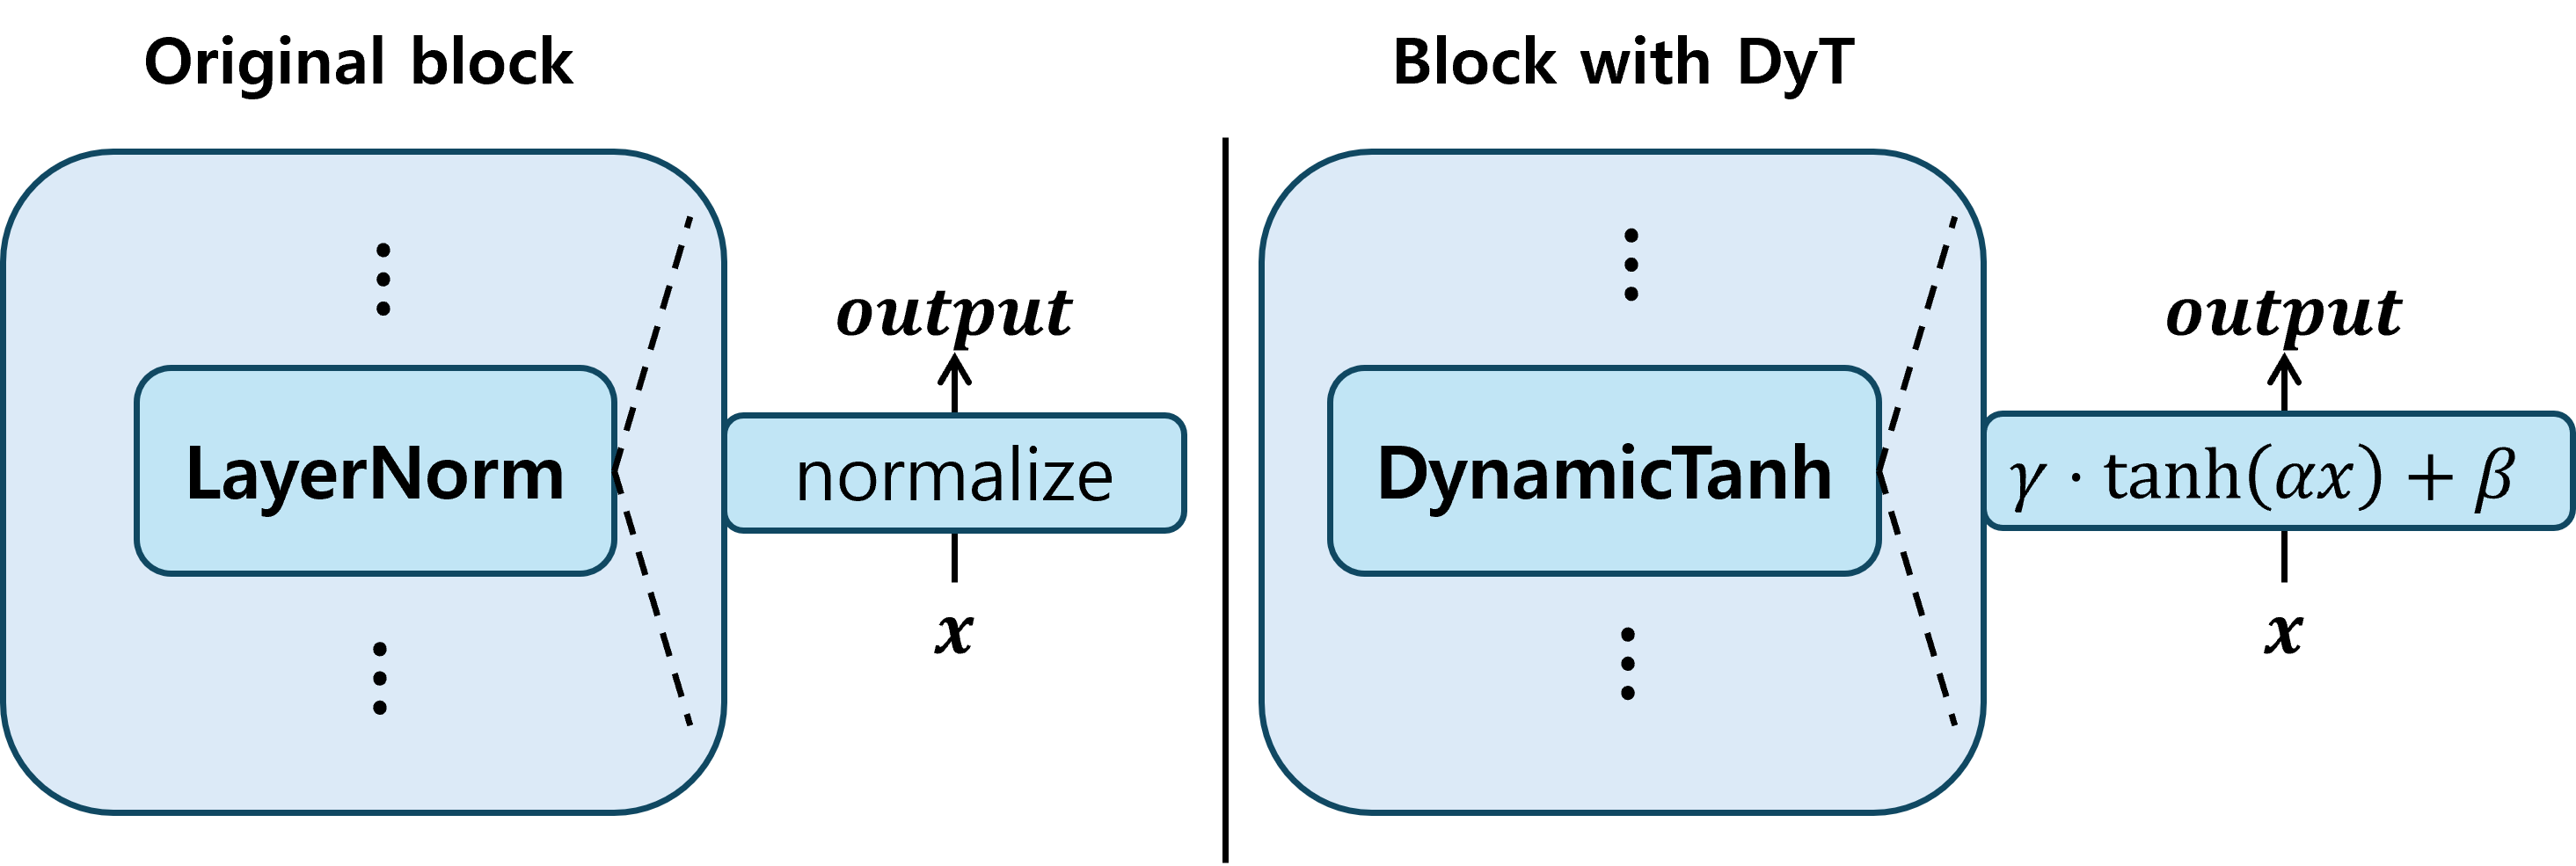
\includegraphics[width=1\linewidth]{figure_dyt.png}
    \caption{\textit{Left}: original Transformer block with LayerNorm. \textit{Right}: block with DyT layer. DyT can be substituted for the commonly used LayerNorm. Our experiments reveal that Transformer with DyT exceed the time efficiency of their LayerNorm counterpart.}    \label{fig:layernorm_decoder}
\end{figure}

\subsection{Transformers}
The Transformer, proposed by Vaswani \textit{et al.} in 2017 \cite{vaswani2017attention}, has shown SOTA performance in sequence-to-sequence tasks, particularly in machine translation. The Transformer handles long-range dependencies within the input sequence using only a self-attention mechanism, without relying on recurrence neural networks (RNNs). This design facilitates parallel processing, significantly enhancing computational efficiency compared to sequential models like seq2seq. \cite{sutskever2014sequence}

\subsubsection{Self-Attention}

Self-attention is the core mechanism of the Transformer. Each token in the input sequence is transformed into Query, Key, and Value vectors. The attention weights between each pair of tokens are computed by taking the dot product of Query and Key, and then these weights are multiplied by the Value vectors to obtain a weighted sum, resulting in new representations for each token. In Multi-Head Attention, this process is performed in parallel across multiple "heads" to capture contextual information from various perspectives. The equation for scaled dot-product attention is as follows:

\begin{equation}
    \text{Attention}(Q, K, V) = \text{softmax}\left(\frac{QK^T}{\sqrt{d_k}}\right)V
\end{equation}

where $Q$, $K$, and $V$ are the Query, Key, and Value matrices, respectively, and $d_k$ is the dimension of the Key vectors.

\subsection{Layer Normalization (LayerNorm)}
Layer Normalization (LayerNorm) \cite{ba2016layer} is a technique proposed to stabilize and accelerate the training of neural networks. LayerNorm normalizes the inputs within each training sample by computing the mean and variance across the neurons in a layer. The formulas are given as follows:

\begin{align*}
\textbf{Mean:} \quad \mu &= \frac{1}{H} \sum_{i=1}^{H} x_i \\
\textbf{Variance:} \quad \sigma^2 &= \frac{1}{H} \sum_{i=1}^{H} (x_i - \mu)^2 \\
\textbf{LayerNorm:} \quad  y_i &= \gamma \frac{(x_i - \mu)}{\sqrt{\sigma^2 + \epsilon}} + \beta
\end{align*}

where $H$ is the number of neurons in the hidden layer, $\gamma$ and $\beta$ are learnable parameters, and $\epsilon$ is a small constant. LayerNorm does not depend on the batch dimension, making it effective for small batch sizes and even recurrent structures.

\subsection{Dynamic Tanh (DyT)}
DyT \cite{zhu2025transformers} is an operation designed as a replacement for LayerNorm layers in neural networks. The development of DyT is motivated by the observed similarity between the output patterns of LayerNorm layers and the shape of a scaled tanh function. Given an input tensor $x$, the DyT layer is defined by the following equation:

\begin{equation}
    \text{DyT}(x) = \gamma \cdot \tanh(\alpha x) + \beta
\end{equation}

In this formulation:

\begin{itemize}
    \item $\alpha$ is a learnable scalar parameter. It plays a crucial role in enabling the input to be scaled differently depending on its range, thereby accommodating varying scales of $ x$. This adaptive scaling is the reason behind the name "Dynamic" Tanh.
    \item  $\gamma$ and $\beta$ are learnable, per-channel vector parameters, mirroring those used in standard normalization layers. These parameters serve the purpose of allowing the output to be rescaled to any desired scale.
\end{itemize}.

\begin{figure}
    \centering    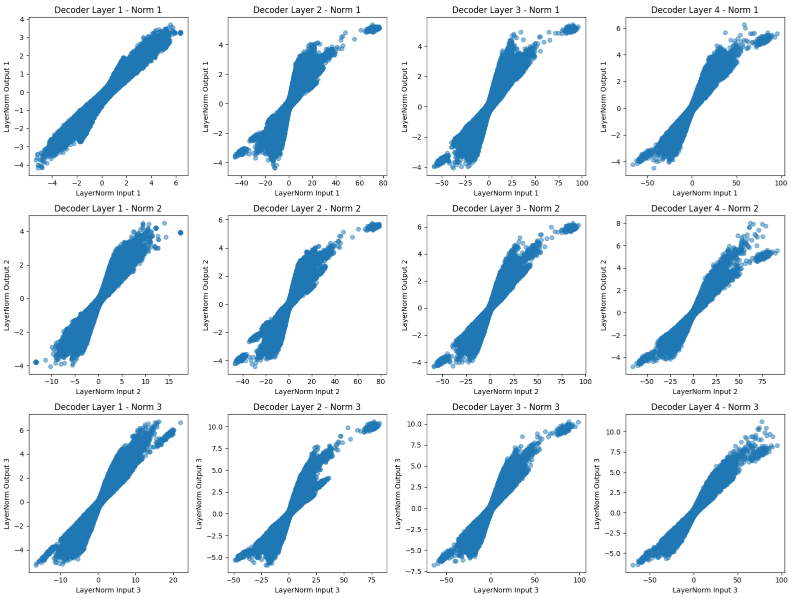
\includegraphics[width=1\linewidth]{figure_layernorm_decoder.png}
    \caption{To illustrate the output characteristics of LayerNorm, we sampled a mini-batch and plotted the input against the output for four different LayerNorm layers. The resulting S-shaped curves strongly resemble the form of a tanh function (as shown in Figure \ref{fig:tanh}). Notably, the more linear patterns observed in earlier layers can also be effectively represented by the central, near-linear portion of a tanh curve. This observation motivates our proposal of Dynamic Tanh (DyT) as a replacement in the Korean-text case.}    \label{fig:layernorm_decoder}
\end{figure}

\section{Can DynamicTanh (DyT) replace LayerNorm?}

This chapter presents the rationale for using Dynamic Tanh (DyT) as a replacement for LayerNorm in the Transformer model and briefly describes the model architectures used in the experiments. As proposed by \cite{zhu2025transformers}, DyT exhibits a consistent similarity to the tanh shape, as observed in 2D image data-based self-supervised learning and diffusion models. (See figure 2 in \cite{zhu2025transformers}.) Figure 3.1 shows the output distribution of LayerNorm after passing through several layers of the Transformer decoder for the Korean question-answering dataset. As can be seen in the figure, the output distribution of LayerNorm closely resembles the shape of a tanh function. Although most of the data distribution falls within the linear region, it can be observed that some data distribution exists in the non-linear regions of tanh. This observation suggests that the role of LayerNorm within the Transformer is to adjust the input values to a specific range and impart non-linearity. In particular, the similarity of the output distribution to the tanh function implies that an operation based on the tanh function could effectively replace the functionality of LayerNorm.

To verify the effectiveness of DyT, this study compares the performance of a baseline model using LayerNorm with a model using DyT under the same Transformer architecture and hyperparameter settings. The basic Transformer architecture of both models is the same as described in the previous chapter, with the only difference being the replacement of the internal LayerNorm layers with DyT layers. The next chapter will present the experimental results of training these models on the Korean question-answer dataset, followed by a comparative analysis of their BLEU scores and training/evaluation times.


\begin{figure}
    \centering
    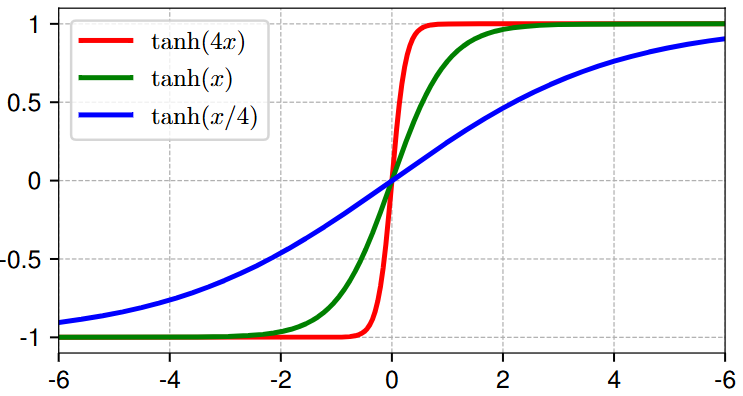
\includegraphics[width=0.5\linewidth]{figure_tanh_function.png}
    \caption{The tanh($\alpha x$) function with different $\alpha$ values.}    \label{fig:tanh}
\end{figure}

\section{Experiments}
This section presents the experimental results of the LayerNorm-based Transformer model and the DyT-based Transformer model trained using a Korean question-answer dataset. Performance was evaluated using the BLEU score, and model efficiency was compared by measuring training and evaluation times.

\subsection{Experimental Setup}
\subsubsection{Dataset}
In this study, we used a publicly available Korean question-answering dataset (\url{https://github.com/songys/Chatbot_data/ChatbotData.csv}) for training.

\subsubsection{Data Augmentation}
To improve the generalization performance of the model, we applied data augmentation techniques. Specifically, we used the following methods:

\begin{itemize}
    \item \textbf{Lexical Substitution:} We replaced words based on their semantic similarity using a pre-trained Korean text embedding model (FastText) provided by Facebook (\url{https://dl.fbaipublicfiles.com/fasttext/vectors-crawl/cc.ko.300.bin.gz}).
    \item \textbf{Random Insertion/Deletion:} We augmented the data by randomly inserting or deleting words at arbitrary positions within the text. The words chosen for random insertion are those with the highest cosine similarity. 
\end{itemize}

\subsubsection{Evaluation Metrics}
The performance of the models was evaluated using the BLEU (Bilingual Evaluation Understudy) score \cite{papineni2002bleu}, a metric widely used in the field of NLP. The BLEU score measures the similarity between the text generated by the model and the reference text written by humans.

\begin{figure}[h!]
    \centering
    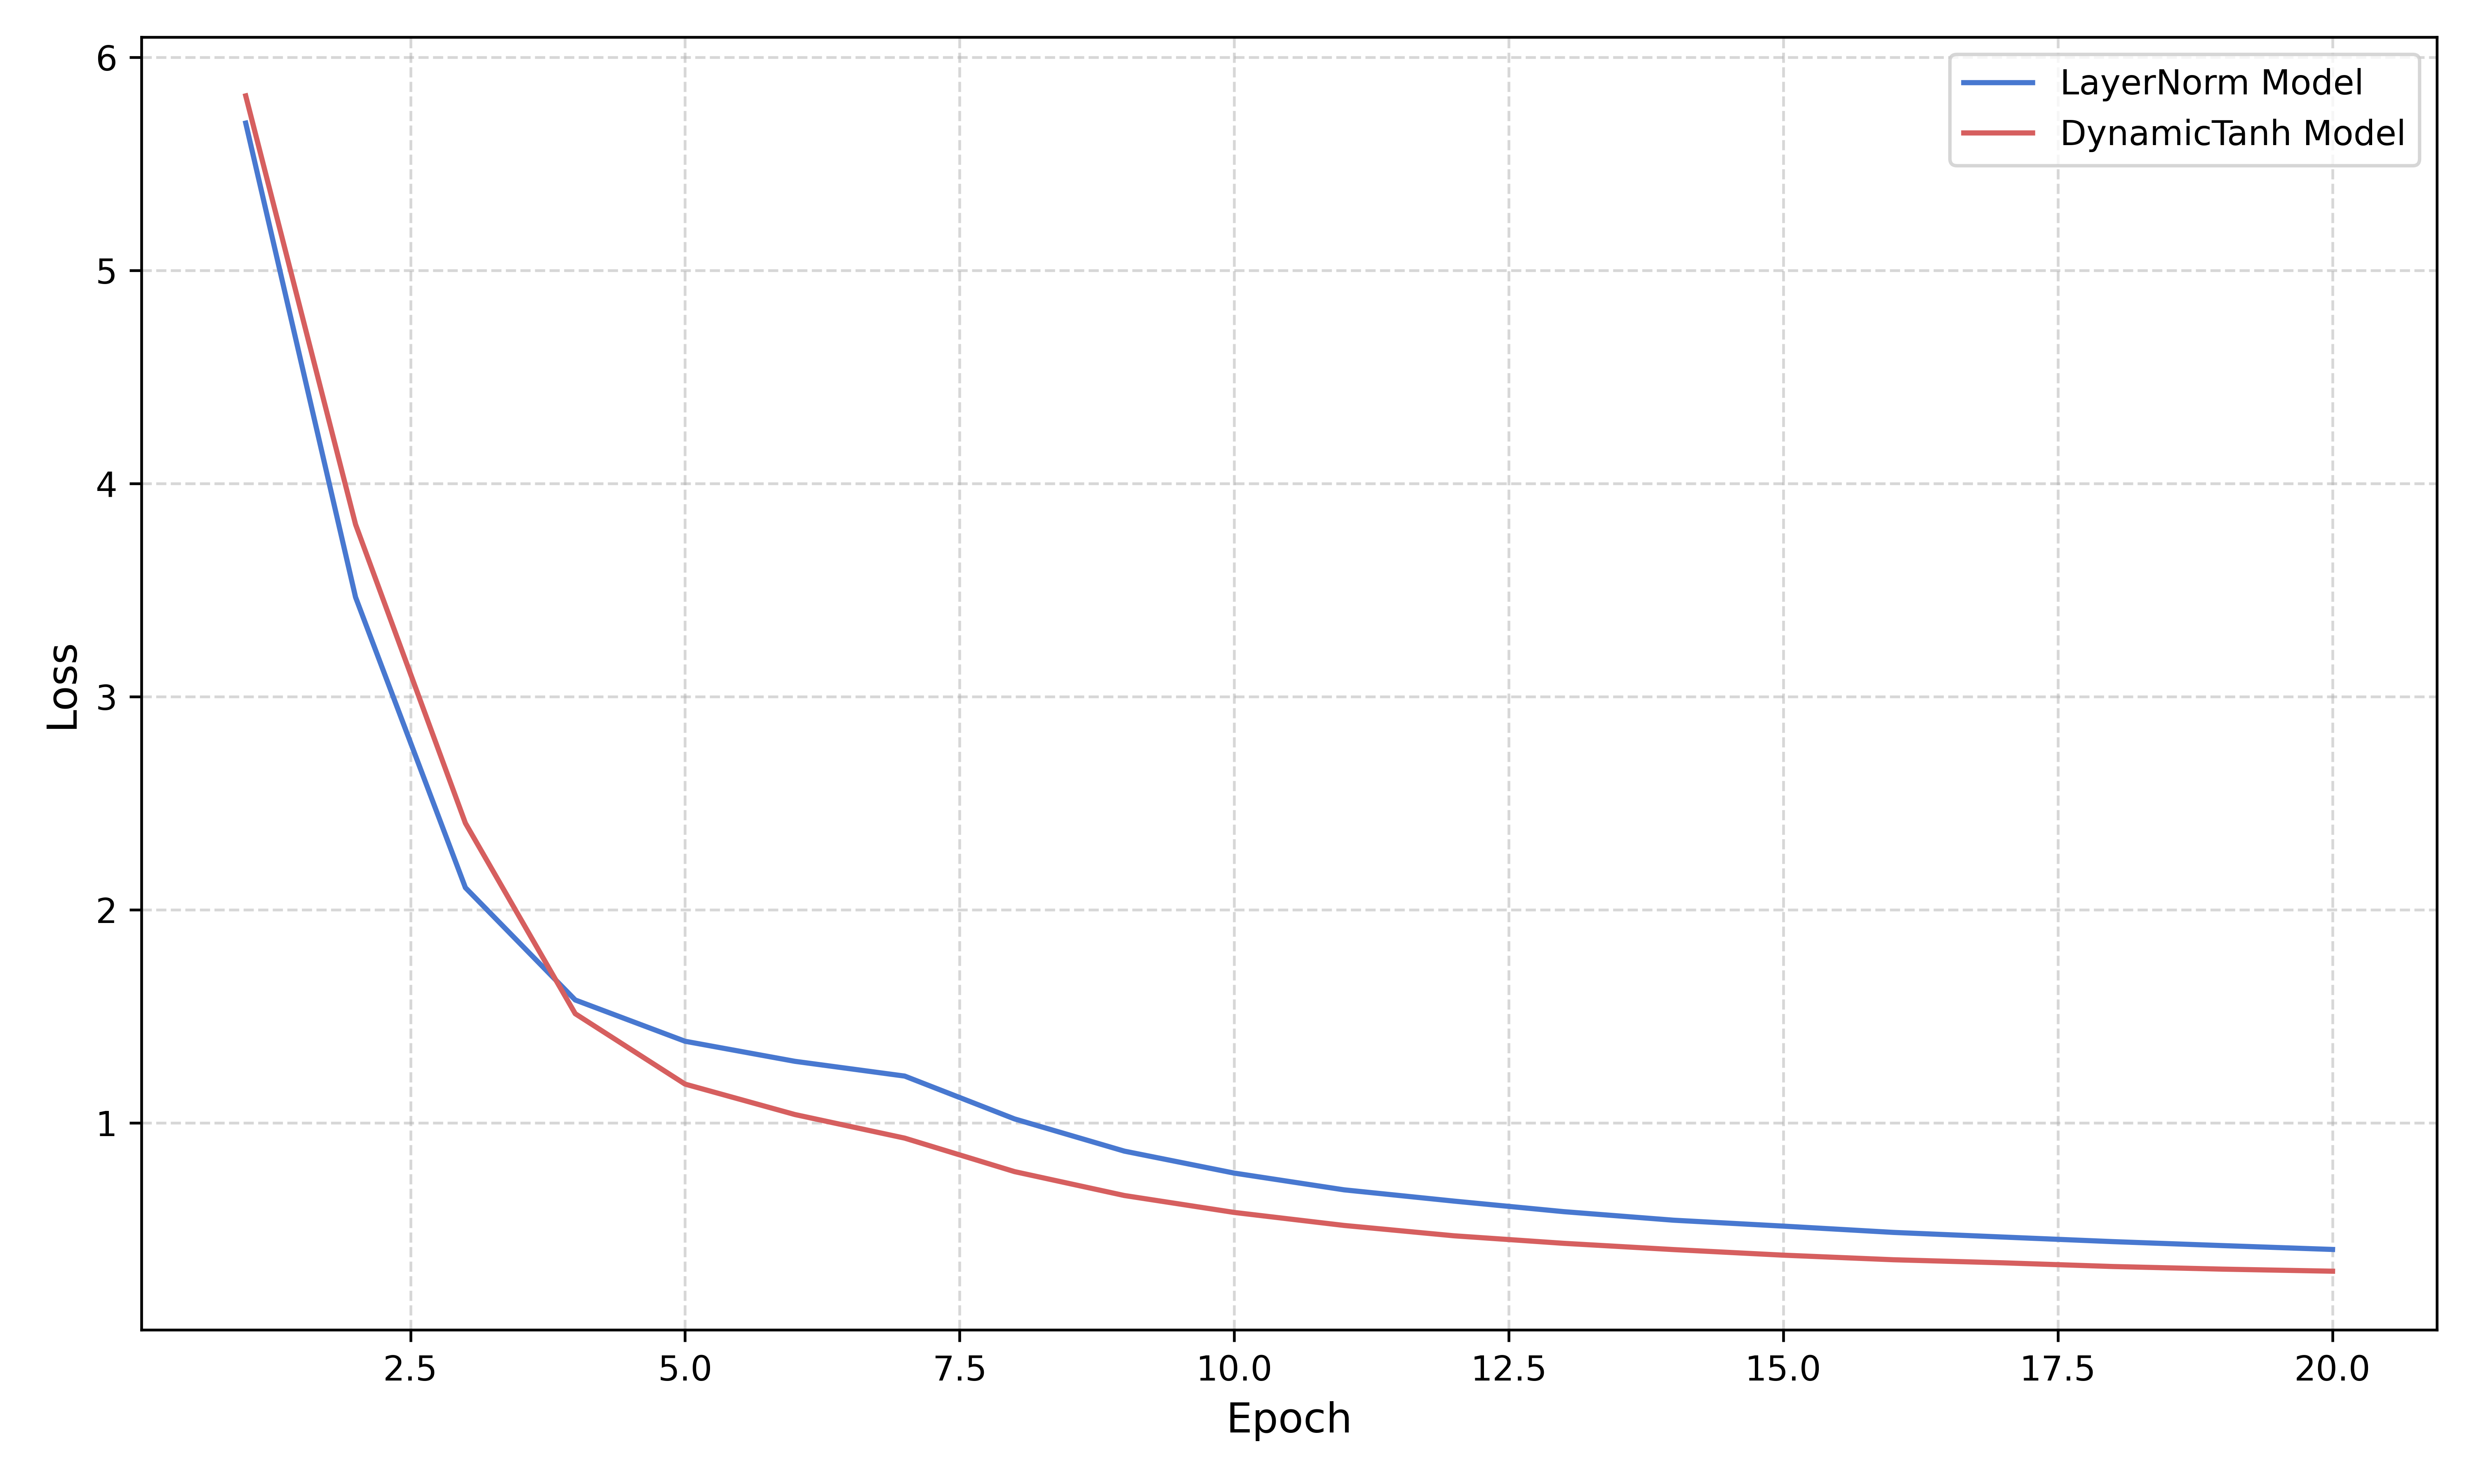
\includegraphics[width=1\textwidth]{figure_loss_dynamics.png}
    \caption{Loss dynamics of LayerNorm-based and DynamicTanh-based models during training.}
    \label{fig:loss_dynamics}
\end{figure}

\begin{center}
\begin{table}
\caption{Comparison of average BLEU scores, execution times, and iterations per second for LayerNorm-based and DyT-based models.}
\label{tab:experimental_results}
\begin{tabular}{lccc}
\toprule
Model & Average BLEU Score & Execution Time (seconds) & Iterations per second (it/s) \\
\midrule
LayerNorm & 64.70 & 88.88 & 6.27 \\
DyT & 64.64 & 74.47 & 8.03 \\
\bottomrule
\end{tabular}
\end{table}
\end{center}

\subsection{Results}
We evaluated the performance and efficiency of LayerNorm and Dynamic Tanh (DyT) within our Transformer model on a randomly selected subset (n=100) of the training data. The DyT model achieved a comparable average BLEU score to the LayerNorm model, indicating successful replacement. However, DyT exhibited a significant advantage in terms of efficiency, demonstrating a 15\% faster execution time and a greater number of iterations per second. The similar learning curves observed in Figure \ref{fig:loss_dynamics} further support the capability of DyT as a practical replacement. These findings suggest that DyT offers a computationally more efficient approach for Korean chatbot development using Transformers, without compromising performance.

\section{Why is it More Efficient?}

The experimental results demonstrate a remarkable observation: the DyT-based model exhibits an approximately 15\% faster execution time compared to the LayerNorm-based model. This enhancement in time efficiency can be attributed to several key factors:

\begin{itemize}
    \item LayerNorm involves statistical calculations for each input sample, including multiple binary operations. In contrast, DyT consists of a simple tanh operation. This difference in complexity may contribute to higher computational efficiency. The square root operation in LayerNorm, similar to division, is also computationally expensive. The element-wise independent operations of DyT are highly suitable for parallel processing, whereas statistical calculations can limit element-wise parallelism.
    \item The tanh function, a widely used activation function, has highly optimized implementations in deep learning frameworks. These optimizations can also contribute to faster operation for DyT.
\end{itemize}

\section{Chapter 6: Conclusion}

This study explored replacing LayerNorm with DynamicTanh (DyT) in a Transformer-based Korean chatbot. Experiments on a Korean question-answer dataset showed DyT achieved comparable BLEU scores to LayerNorm, validating its performance-preserving capability. DyT reduced training and evaluation time by approximately 15\%, indicating improved efficiency. These results suggest that DyT is a promising alternative to improve the efficiency of Transformer-based Korean chatbots without harming performance. Future research could explore the DyT performance across diverse Korean NLP tasks and larger datasets, and analyze its impact in various Transformer architectures. In conclusion, DyT shows significant potential as an efficient substitute for LayerNorm in Transformer-based Korean chatbot models.

\bibliographystyle{plain}\bibliography{references}

\section*{Appendix}

\subsection{Hyperparameters}
The hyperparameters used for the Transformer model in this study are detailed in Table \ref{tab:model_hyperparameters}.

\begin{center}
\begin{table}
\caption{Model Hyperparameters}
\label{tab:model_hyperparameters}
\begin{tabular}{lc}
\toprule
Hyperparameter & Value \\
\midrule
Total dataset size(augmented) & 24770 \\
Number of layers (n\_layers) & 4 \\
Model dimension (d\_model) & 256 \\
Number of attention heads (n\_heads) & 4 \\
Feed-forward network dimension (d\_ff) & 1024 \\
Dropout rate & 0.5 \\
Vocabulary size (vocab\_size) & 15000 \\
Maximum positional length (pos\_len) & 50 \\
Batch size & 32 \\
Number of epochs & 20 \\
\bottomrule
\end{tabular}
\end{table}
\end{center}

\subsection{Encoder LayerNorm Output}

\begin{figure}[h!]
    \centering
    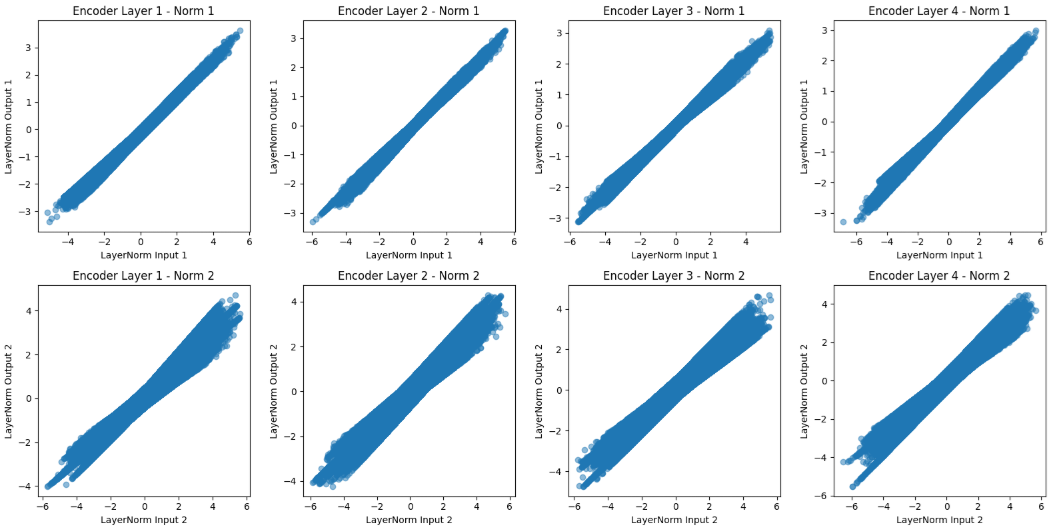
\includegraphics[width=1\textwidth]{figure_layernorm_encoder.png}
    \caption{LayerNorm output of the encoder part.}
    \label{fig:layernorm_encoder}
\end{figure}

Figure \ref{fig:layernorm_encoder} illustrates the LayerNorm output of the encoder part. Most of the data points are located in the linear region, which can be captured by the central part of a tanh curve.

\subsection{Text Generation Examples}

Table \ref{tab:text_generation_examples} provides examples of text generation results from the LayerNorm-based model and the DyT-based model.

\begin{center}
\begin{table}
\caption{Text Generation Examples}
\label{tab:text_generation_examples}
\begin{tabular}{llp{8cm}}
\toprule
Example Sentence & LayerNorm Model Sequence & DyT Model Sequence \\
\midrule
지루하다, 놀러가고 싶어. & 재미 가 있 을 거 예요 & 저도 놀 고 싶 어요 \\
오늘 일찍 일어났더니 피곤하다. & 시간 이 좀 생길 거 예요 & 더 잠 드 는 건 어때 요 \\
간만에 여자친구랑 데이트 하기로 했어. & 울 고 있 을 거 예요 & 잘 놀아 요 \\
집에 있는다는 소리야. & 집 에 비밀 은 시간 이 에요 & 뭐 라도 하 세요 \\
비가 와서 그런가 기분이 좀 별로야. & 감성 적 이 기 딱 좋 죠 & 감성 적 이 에요 \\
\bottomrule
\end{tabular}
\end{table}
\end{center}






\end{document}